\begin{displayquote}
	\textsf{Many problems in science and engineering often require to solve simultaneously large-scale non-Hermitian sparse linear systems with multiple right-hand sides (RHSs). Efficiently solving such problems on extreme-scale platforms also requires the minimization of global communications, reduction of synchronization points and promotion of asynchronous communications. UCGLE is also a suitable candidate with the reduction of global communications and the synchronization points of all computing units. In this chapter, we develop another extension of UCGLE method by combining it with block GMRES method to solve non-Hermitian linear systems with multiple RHSs, with novel designed manager engine implementations. This engine is capable of allocating multiple BGMRES at the same time, each Block GMRES solving the linear systems with a subset of RHSs and accelerating the convergence using the eigenvalues approximated by other eigensolvers. Dividing the entire linear system with multiple RHSs into subsets and solving them simultaneously with different allocated linear solvers allow localizing calculations, reducing global communication, and improving parallel performance. Meanwhile, the asynchronous preconditioning using eigenvalues can speed up the convergence and improve the fault tolerance and reusability. Numerical experiments using different test matrices on supercomputer ROMEO indicate that the proposed method achieves a substantial decrease in both computation time and iterative steps with good scaling performance.}
\end{displayquote}

\vspace{0.6in}

\section{Demand to Solve Linear Systems with Multiple Right-hand-sides}

In this chapter, we consider solving the system

\begin{equation}
\label{AX=B}
AX =  B,
\end{equation}
where $A \in$ $\mathbb{C}^{n \times n}$ is a large, sparse and non-Hermitian matrix of order $n$, $X=[x_1,\cdots,x_s] \in$  $\mathbb{C}^{n \times s}$ and $B=[b_1,\cdots,b_s] \in$  $\mathbb{C}^{n \times s}$ are rectangular matrices of dimension $n \times s$ with $s \leq n$. In this paper, the rectangular matrices such as $B$ is also called multi-vector, which can be seen as the combination of $s$ vectors $b_i$ $\forall i \in 1, 2, \cdots, s$. This kind of linear systems with multiple RHSs arise from a variety of applications in different scientific and engineering fields, such as the QCD \cite{sakurai2010application, nakamura2012modified, fiebach1997variants}, the wave scattering and propagation simulation \cite{malhotra1997iterative}, dynamics of structures \cite{barbella2011block, ferraz2001block, nour1985short}, etc. The block Krylov methods are good candidates if we want to solve these large linear systems at the same time because the block methods can expand the search space associated with each RHS and may accelerate the convergence. Another feature of block Krylov methods is that they can be implemented using BLAS3, which improves the locality and reusability of data and reduces the memory requirement on modern computer architectures \cite{agullo2014block}. The block Krylov methods replace the SpMV in each iterative step of the conventional Krylov methods with the SpGEMM.


\section{Block GMRES Method}

This section introduces the details of block Krylov subspace and block GMRES to solve linear systems with multiple RHSs.

\subsection{Block Krylov Subspace}

In linear algebra, the $m$-order Block Krylov subspaces $K_{m\times s}^{\square}$ \cite{gutknecht2006block} generated by an operator matrix $A \in \mathbb{C}^{n\times n}$ and a vector $B \in \mathbb{C}^{n\times s}$ 

\begin{equation}
K_{m\times s}^{\square}(A,B)=\textit{Block span}\{B, AB, \cdots, A^{n-1}B\} \in \mathbb{C}^{N \times s},
\end{equation}

A block Krylov subspace method for solving the linear systems (\ref{AX=B}) is an iterative method that generates an approximate solution $X_n$ such that

\begin{equation}
	X_n-X_0 \in K_{m\times s}^{\square}(A,R_0),
\end{equation}

where $R_0=B-AX_0$ is the initial guess residual. For each RHS $b^{(i)}$ with $i \in 1, 2, \cdots, s$, its Krylov subspace generated by the block operation of $A$ and $B$ can be defined as

\begin{equation}
\begin{aligned}
	K_{m\times s}(A,B) &= K_{m}(A,b^{(1)})+\cdots+ K_{m}(A,b^{(s)}) \\
&=Span\{b_0^{(1)},\cdots,b_0^{(s)}, Ab_0^{(1)},\cdots,Ab_0^{(s)},\cdots,A^{m-1}b_0^{(1)},\cdots,A^{m-1}b_0^{(s)} \}.
\end{aligned}
\end{equation}

Thus $K_{m\times s}^{\square}(A,B)$ is just the Cartesian product of $s$ copies of $K_{m\times s}$

\begin{equation}
\begin{aligned}
	K_{m\times s}^{\square}&=\bigtimes_{s\text{ times}}K_{m\times s}.
\end{aligned}
\end{equation}

Thus $x_0^{(i)}+K_{m\times s}$ is the affine space where the approximation solution $x_n^{(i)}$ of the solution of the $i$-th systems $Ax^{(i)}=b^{(i)}$ is constructed from

\begin{equation}
	x_m^{(i)} \in x_0^{(i)} + K_{m\times s}.
\end{equation}

Clearly, if all the $ms$ vectors $A^{k}b^{(i)} \in \mathbb{C}^{n}$ are linearly independent,

\begin{equation}
	\textit{dim }  K_{m\times s} = ns.
\end{equation} 

But this may not always be true, especially for different $b^{(i)}$ that are correlated. However even for the case that $\textit{dim }  K_{m\times s} < ns$, the searching space for each RHS $b^{(i)}$ can be enlarged, and a potential acceleration might be achieved. More exactly: block methods are most effective if

\begin{equation}
	\textit{dim } K_{m\times s} (A, R_0) \ll \sum_{k=1}^{s} \textit{dim } K_{m} (A, r_0^{(k)}).
\end{equation}

\subsection{Block Arnoldi Reduction}

In this section, we introduce the block version of Arnoldi reduction. Firstly, we define \textit{block-orthogonal} and \textit{block-normalized}. Denote the zero and unit matrix in $\mathbb{C}^{s \times s}$ by $o$ and $\iota$. The block vectors $X$ and $Y \in \mathbb{C}^{n \times s}$ is \textit{block-orthogonal} if $X*Y=o$, and we call $X$ \textit{block-normalized} if $X*X=\iota$. A set of block vectors $\{X_n\}$ is block orthonormal if these block vectors are block-normalized and mutually block-orthogonal. So, a set of block-orthonormal block vectors has the property that all the columns in this set are normalized N-vectors that are orthogonal to each other (even if they belong to the same block).

For matrix $A \in \mathbb{C}^{N \times N}$ and $V \in \mathbb{C}^{N \times s}$, a block Arnoldi reduction is able to generate nested block-orthonormal basis for the block Krylov subspace $K_{m\times s}^{\square} (A,V)$. Each column in the basis of $K_{m\times s}^{\square} (A,V)$  form at the same time an orthonormal basis of at most $ns$-dimensional space $K_{m\times s}(A,V)$. A version of block Arnoldi reduction with modified Gram-Schmit orthogonalization is given as Algorithm \ref{alg:block arnoldi}. The initialization step with a QR factorization generate an orthonormal baisis of $K_{1\times s}$ as $V_0$. For the subsequent $m$ steps yield nests orthonormal bases for  $K_{2\times s}, \cdots,K_{{(m+1)}\times s}$. 

\begin{algorithm}[htbp]
	\caption{Block Arnoldi Algorithm}   
	\label{alg:block arnoldi}   
	\begin{algorithmic}[1]
		\Function {Block Arnoldi}{$input$:$A,m,V \in \mathbb{C}^{N\times s}$ of full rank, $output$: $H_m, \Omega_m$}
		\State $V_0P_0 := V$ \Comment{QR factorization: $P_0 \in \mathbb{C}^{s\times s}, V_0 \in \mathbb{C}^{N \times s},  V_0^* V_0=I$}
		\For {\texttt{$j=0,1, 2, \cdots, m$}}
		\State $U_j = AV_{j}$  \Comment{$s$ MVs}
		\For {$i = 1,2,4,\cdots, j$}
		\State $H_{i,j} = V_i^T U_j$ \Comment{$s^2$ SDOTs}
		\State $U_j = U_j - V_iH_{i,j}$ \Comment{$s^2$ SAXPYs}
		\EndFor
		\State $U_j = V_{j+1}H_{j+1,j}$  \Comment{QR factorization: $H_{j+1,j} \in \mathbb{C}^{s\times s}, V_{j+1} \in \mathbb{C}^{N \times s},  V_{j+1}^* V_{j+1}=I$}
		\EndFor 
		\EndFunction
	\end{algorithmic}  
\end{algorithm}

Then we define the $N\times m$ matrices
\[\bar{V}_m = (V_0 \quad V_1  \quad \cdots  \quad V_{m-1})\]

and the $(m+1)s \times ms$ matrix as Fig. \ref{fig:block-hessemberg}, with block matrix $H_{1,0}, \cdots, H_{m,m-1}$ in the band to be upper triangale. 

\begin{figure}[htbp]
	\centering
	\includegraphics[width=0.6\linewidth]{fig/block-hessemberg.pdf}
	\caption{Structure of block Hessenberg matrix.}
	\label{fig:block-hessemberg}
\end{figure}

Finally the Arnoldi relation can be obtained as:

\begin{equation}
\label{blockarnoldi}
	AV_m= V_{m+1} \underline{H}_m.
\end{equation}

\subsection{Block GMRES Method}

The BGMRES is constructed based the block Arnoldi reduction (shown as Algorithm \ref{alg:block arnoldi}) to solve the linear systems with multiple RHSs. Similar with the standard GMRES, BGMRES starts with a given initial guess solution $\in \mathbb{C}^{N\times s}$ of Equation (\ref{AX=B}), the related residual is of form

\begin{equation}
	R_0=B-AX_0
\end{equation}

The temporary solution $X_n$ in the $n$-dimensional block Krylov subspace is

\begin{equation}
	X_n = X_0+V_nY_n,
\end{equation}

and the $n$-th block residual vector $R_n$ can be obtained as 

\begin{equation}
	R_n= B-AX_n=R_0-AV_nY_n
\end{equation}

With the relation (\ref{blockarnoldi}) of Arnoldi reduction, and $R_0=V_{n+1}e_1P_0$, we have

\begin{equation}
	R_n=V_{n+1}(\underline{e_1}P_0-\underline{H}_nY_n).
\end{equation}

where
\begin{itemize}
	\item $\underline{e_1}$ the first $s$ columns of the $(n+1)s \times (n+1)s$ unit matrix,
	\item $P_0 \in \mathbb{C}^{s \times s}$ upper triangular, obtained in Arnoldi's initializtion step,
	\item $\underline{H}_n$ the leading $(n+1)s \times ns$ submatrix of $\underline{H}_m$,
	\item $Y_n \in \mathbb{C}^{ns \times s}$ the "block coordianates" of $X_n-X_0$,
\end{itemize}

In order to get $Y_n$, a least squares problem should be solved
\begin{equation}
\label{blockgmresls}
	\textit{min} ||R_n||_F \text{ with } X_n-X_0 \in K_{m\times s}^{\square}.
\end{equation}

where the operation $||.||_F$ for a block vector $Q \in \mathbb{C}^{N \times s}$ is defined as

\begin{equation}
	||Q||_F=\sqrt{\sum_{j=1}^{s}||x^{(j)}||_2^2}==\sqrt{\sum_{j=1}^{s}\sum_{i=1}^{N}|x_i^{(j)}|^2}.
\end{equation}

But this least square problem is equivalent to
\begin{equation}
	\textit{min} ||r_n^{(i)}||_2 \text{ with } x_n^{(i)}-x_0^{(i)} \in K_{m\times s}, \forall i=1,2,\cdots,s.
\end{equation}

Since $V_n$ has orthonormal columns, finally, we have

\begin{equation}
	\textit{min} ||\underline{e_1}p_0^{(i)}-\underline{H}_ny_n^{(i)}||_2 \text{ with } y_n^{(i)} \in \mathbb{C}^{ns}, \forall i=1,2,\cdots,s.
\end{equation}

These $s$ least squares problems with the same matrix  $\underline{H}_n$ can be solved efficiently by recursivelt computing the QR factorization of $\underline{H}_n$. An example of BMGRES is shown as Algorithm \ref{alg:block gmres}.
 
\begin{algorithm}[htbp]{}
	\caption{Block GMRES Algorithm}   
	\label{alg:block gmres}   
	\begin{algorithmic}[1]
		\Function {Block GMRES}{$input$:$A,m,B, X_0\in \mathbb{C}^{N\times s}$ of full rank, $output$: $X$}
		\State $R = B - AX_0$
		\State $V_0R_0 := R$ \Comment{QR factorization: $P_0 \in \mathbb{C}^{s\times s}, V_0 \in \mathbb{C}^{N \times s},  V_0^* V_0=I$}
		\For {\texttt{$j=0,1, 2, \cdots, m$}}
		\State $U_j = AV_{j}$  \Comment{$s$ MVs}
		\For {$i = 1,2,4,\cdots, j$}
		\State $H_{i,j} = V_i^T U_j$ \Comment{$s^2$ SDOTs}
		\State $U_j = U_j - V_iH_{i,j}$ \Comment{$s^2$ SAXPYs}
		\EndFor
		\State $U_j = V_{j+1}H_{j+1,j}$  \Comment{QR factorization: $H_{j+1,j} \in \mathbb{C}^{s\times s}, V_{j+1} \in \mathbb{C}^{N \times s},  V_{j+1}^* V_{j+1}=I$}
		\EndFor
		\State $W_m = [V_1, V2, \cdots, V_m]$, $H_m = \{H_{i,j}\}_{0 \leq i \leq j; 1 \leq j \leq m}$ 
		\State Find $y_m$, s.t. $||\beta - H_my_m||_2$ is minimized
		\State $X = X + W_my_m$
		\EndFunction
	\end{algorithmic}  
\end{algorithm}

\subsection{Cost Comparison}

In this section, we list the computational cost of the block Arnoldi process and BGMRES, and compare it with the cost of solving each system separately.

Here is a table of the cost of m steps of block Arnoldi compared with $s$ times the cost of $m$ steps of (unblocked) Arnoldi. Clearly, block Arnoldi is more costly than $s$ times Arnoldi.

\begin{table}[htbp]
	\renewcommand{\arraystretch}{1.4}
	\small	
	\caption{Operation Cost \cite{gutknecht2006block}.}
	\label{block-arnoldi}
	\centering
	\begin{tabular}{c|c|c}
		\toprule
		\cellcolor{gray!50}Operations & \cellcolor{gray!50}Block Arnoldi & \cellcolor{gray!50}$s$ times Arnoldi  \\
		\midrule
		MVs  & $ms$ & $ms$ \\
		\cellcolor{gray!20}SDOTs & \cellcolor{gray!20}$\frac{1}{2}m(m+1)s^2+\frac{1}{2}ms(s+1)$ & \cellcolor{gray!20}$\frac{1}{2}m(m+1)s$   \\
		SAXPYs & $\frac{1}{2}m(m+1)s^2+\frac{1}{2}ms(s+1)$ & $\frac{1}{2}m(m+1)s$ \\
		\bottomrule
	\end{tabular}
\end{table}

The next table shows the storage requirements of $m$ steps of block Arnoldi compared with those of $m$ steps of Arnoldi (applied once):

\begin{table}[htbp]
	\renewcommand{\arraystretch}{1.4}
	\small	
	\caption{Storage Requirement \cite{gutknecht2006block}.}
	\label{block-arnoldi-memory}
	\centering
	\begin{tabular}{c|c|c}
		\toprule
		\cellcolor{gray!50}Operations & \cellcolor{gray!50}Block Arnoldi & \cellcolor{gray!50}$s$ times Arnoldi  \\
		\midrule
		$y_0,\cdots,  y_m$ & $ms(s+1)N$ & $(m+1)N$   \\
		\cellcolor{gray!20}$\rho_0,H_m$ & \cellcolor{gray!20}$\frac{1}{2}s(s+1)+\frac{1}{2}ms(ms+1)+ms^2$ & \cellcolor{gray!20}$1+\frac{1}{2}m(m+1)+m$ \\
		\bottomrule
	\end{tabular}
\end{table}

If we apply (unblocked) Arnoldi $s$ times, we can always use the same memory if the resulting orthonormal basis and Hessenberg matrix need not be stored. However, if we distribute the $s$ columns of $V_0$ on $s$ processors with attached (distributed) memory, then block Arnoldi requires a lot of communication.

The extra cost of m steps of BGMRES on top of block Arnoldi compared with $s$ times the extra cost of $m$ steps of GMRes is given in the following table:

\begin{table}[htbp]
	\renewcommand{\arraystretch}{1.4}
	\small	
	\caption{Extra cost of Block GMRES comparing with $s$ times GMRES \cite{gutknecht2006block}.}
	\label{block-gmres-extra}
	\centering
	\begin{tabular}{c|c|c}
		\toprule
		\cellcolor{gray!50}Operations & \cellcolor{gray!50}Block GMRES & \cellcolor{gray!50}$s$ times GMRES  \\
		\midrule
		MVs  & $s$ & $s$ \\
		\cellcolor{gray!20}SDOTs & \cellcolor{gray!20}$ms^2$ & \cellcolor{gray!20}$ms$   \\
		scalar work & $\mathcal{O}(m^2s^3)$ & $\mathcal{O}(m^s)$ \\
		\bottomrule
	\end{tabular}
\end{table}

In particular, in the $(k+1)$-th block step we have to apply first $ks^2$ Givens rotations to the $k$-th block column (of size $(k+1)s\times s$) of $\underline{H}_m$, which requires $\mathcal{O}(ks^3)$ operations. Summing up over $k$ yields $\mathcal{O}(m^2s^3)$ operations. Moreover, $s$ times back substitution with a triangular $ms \times ms$ matrix requires also $\mathcal{O}(m^2s^3)$ operations.

Let us summarize these numbers and give the mean cost per iteration of BGMRES compared with $s$ times the mean cost per iteration of GMRES:

\begin{table}[htbp]
	\renewcommand{\arraystretch}{1.4}
	\small	
	\caption{Extra cost of Block GMRES comparing with $s$ times GMRES. \cite{gutknecht2006block}}
	\label{block-gmres}
	\centering
	\begin{tabular}{c|c|c|c}
		\toprule
		\cellcolor{gray!50}Operations & \cellcolor{gray!50}Block GMRES & \cellcolor{gray!50}$s$ times GMRES & \cellcolor{gray!50}ratio  \\
		\midrule
		MVs  & $(1+\frac{1}{m})s$ & $(1+\frac{1}{m})s$ & 1\\
		\cellcolor{gray!20}SDOTs & \cellcolor{gray!20}$\frac{1}{2}(m+1)s^2+\frac{1}{2}s(s+1)$ & \cellcolor{gray!20}$\frac{1}{2}(m+1)s$ & \cellcolor{gray!20}$s+\frac{s+1}{m+1}$   \\
		SAXPYs &  $\frac{1}{2}(m+3)s^2+\frac{1}{2}s(s+1)$ & $\frac{1}{2}(m+3)s$ & $s+\frac{s+1}{m+3}$ \\
		\cellcolor{gray!20}scalar work & \cellcolor{gray!20}$\mathcal{O}(ms^3)$ & \cellcolor{gray!20}$\mathcal{O}(m^s)$& \cellcolor{gray!20}$\mathcal{O}(s^2)$\\
		\bottomrule
	\end{tabular}
\end{table}

Recall that the most important point in the comparison of block and ordinary Krylov space solvers is that the dimensions of the search spaces $K_{m \times s}$and $K_m$ differ by a factor of up to $s$. This could mean that BGMRES may converge in roughly $s$ times fewer iterations than GMRES. Ideally, this might even be true if we choose

\begin{equation}
	m_{BGMRES} = \frac{1}{s}m_{GMRES}.
\end{equation}

This assumption would make the memory requirement of both methods comparable. Unfortunately, the numerical experiments indicate that it is rare to fully achieve this factor $\frac{1}{s}$.

\subsection{Challenges of Exising Methods for Large-scale Platforms}

However, nowadays, HPC cluster systems continue to scale up not only the number of compute nodes and CPU cores but also the heterogeneity of components by introducing GPUs and many-core processors. This results in the tendency of transition to multi- and many cores within computing nodes, which communicate explicitly through faster interconnection networks. These hierarchical supercomputers can be seen as the intersection of distributed and parallel computing. Indeed, for a large number of cores, the communication of overall reduction operations and global synchronization of applications are the bottleneck. When solving linear systems by block Krylov methods on large-scale distributed memory platforms, the cost of using BLAS3 operations to enlarge search space and reduce the memory requirement is apparent: the communication bound of SpGEMM in each step of Arnoldi projection damages heavily their performance, which cannot be compensated by the advantages of the block methods. Even using classic Krylov methods, such as GMRES, to solve a large-scale problem on parallel clusters, the cost per iteration of them becomes the most significant concern, typically caused by communication and synchronization overheads. Consequently, large scalar products, overall synchronization, and other operations involving communication among all cores have to be avoided. 


\section{$m$-UCGLE for Multiple Right-hand-sides}

We propose to combine the BGMRES \cite{vital1990etude} with UCGLE \cite{wu2018distributed} to solve Equation (\ref{AX=B}) in parallel on modern computer architectures. In this paper, firstly, we develop a block version of Least Squares Polynomial method based on \cite{saad1987least}, then replace the three computing components of UCGLE respectively by the BGMRES, Shifted Krylov-Schur ($s$-KS), and B-LSP. Additionally, in order to solve linear systems with multiple RHSs and reduce the global communication produced by SpGEMM inside block methods, we design and implement a new manager engine to replace the former one in UCGLE. This novel engine allows to allocate and deploy multiple BGMRES and/or $s$-KS Components at the same time and support their asynchronous communications. Each allocated BGMRES is assigned to solve the linear systems with a subset of RHSs. This extension is denoted as multiple-UCGLE or $m$-UCGLE even though the ERAM Component is replaced by $s$-KS method. 

\subsection{Shifted Krylov-Schur Algorithm}

UCGLE uses the dominant eigenvalues to accelerate the convergence of GMRES, and theoretically, the more eigenvalues are applied, the acceleration of Least Squares Polynomial will be more significant \cite{wu2018distributed}.  In order to approximate more eigenvalues by ERAM Component, the easiest way is to enlarge the size of related Krylov Subspace. In $m$-UCGLE, we replace ERAM Component by $s$-KS method which is another variant of the Arnoldi algorithm with an effective and robust restarting scheme and numerical stability \cite{stewart2002krylov}. The Krylov subspace of  $s$-KS cannot be too large. Otherwise BGMRES Component is not able to receive the eigenvalues in time to perform the B-LSP acceleration. With the novel developed manager engine of $m$-UCGLE in this paper, several different $s$-KS components can be allocated at the same time to approximate efficiently the different part of dominant eigenvalues of matrix $A$, by the shift with different values and thickly restarting with smaller Krylov subspace sizes. The algorithm of $s$-KS is given in Algorithm \ref{alg:krylov-schur-2}.

\begin{algorithm}[htbp]{}
	\caption{Shifted Krylov-Schur Method}   
	\label{alg:krylov-schur-2}   
	\begin{algorithmic}[1]
		\Function {$s$-KS}{$input$: $A, x_1, m, \sigma$, $output$: $\Lambda_k$ with $k \leq p$}
		\State $A \leftarrow A-\sigma I$ 
		\State Build an initial Krylov decompostion of order $m$
		\State Apply orthogonal transformations to get a Krylov-Schur decompostion
		\State Reorder the diagonal blocks of the Krylov-Schur decompostion
		\State Truncate to a Krylov-Schur decompostion of order $p$
		\State Extend to a Krylov decomposition of order $m$
		\State If not satisfied, go to step 3
		\EndFunction
	\end{algorithmic}  
\end{algorithm}

\subsection{Least Squares Polynomial for Multiple Right-hand sides}

The Least Squares polynomial method is an iterative method proposed by Saad \cite{saad1987least} to solve linear systems. It is applied to calculate a new preconditioned residual for restarted GMRES in UCGLE. In this section, we will present the B-LSP method, which is a block extension of Least Squares polynomial method to solve linear systems with multiple RHSs at the same time. The iterates of B-LSP method can be written as $X_n=X_0+\mathcal{P}_d(A)R_0$, where $X_0 \in \mathbb{C}^{N\times s}$ is a selected initial guess to the solution, $R_0 \in \mathbb{C}^{N\times s}$ the corresponding residual multi-vector, and $\mathcal{P}_d$ a polynomial of degree \(d-1\). We set a polynomial of $n$ degree $\mathcal{R}_n$ such that \[\mathcal{R}_d(\lambda)=1-\lambda \mathcal{R}_d(\lambda)\].

The residual of \(n^{th}\) steps iteration \(R_n\) can be expressed as equation $R_n=\mathcal{R}_d(A)R_0$, with the constraint \(\mathcal{R}_d(0)=1\). We want to find a kind of polynomial which can minimize all \(||\mathcal{R}_d(A)R_0^{(p)}||_2\), with $p \in 0,1,\cdots,s-1$, $R_0^{(p)}$ the $p^{th}$ vector in the multi-vector $R_0$ and \(||.||_2\) the Euclidean norm.

Suppose $A$ is a diagonalizable matrix with its spectrum denoted as \(\sigma(A)=\lambda_1, \cdots, \lambda_n\), and the associated eigenvectors \(u_1, \cdots, u_n\). Expanding the each component of \(R_n\) in the basis of these eigenvectors as as $R_n^{(p)}=\sum_{i=1}^{n}\mathcal{R}_d(\lambda_i)\rho_i u_i$, which allows to get the upper limit of $||R_n^{(p)}||_2$ with $p \in 0,1,\cdots,s-1$ as:

\begin{equation}
\label{eq113}
||R_0||_F \max_{\lambda \in \sigma(A)}|\mathcal{R}_d(\lambda)|
\end{equation}

In order to minimize the norm of $R_n^{(p)}$, it is possible to find a polynomial $\mathcal{P}_d$ which can minimize the Equation (\ref{eq113}).

Similarly for the Least Squares problem (\ref{blockgmresls}) in block GMRES, this maximum-minmum problem is equivalent to 

\begin{equation}
	||R_0^{(p)}||_2 \max_{\lambda \in \sigma(A)}|\mathcal{R}_d(\lambda)|, \quad \forall p \in 0,1,\cdots,s-1.
\end{equation}

Therefore, for all $s$ linear systems with different RHSs, they share the same best LS polynomial $\mathcal{R}_d$. As presented in Section \ref{Preconditioning by Polynomials - Introduction in detail on Least Squares Polynomial method}, $\mathcal{P}_d$ can be expanded with a basis of Chebyshev polynomial $t_j(\lambda)=\frac{T_j \frac{\lambda-c}{b}}{T_j \frac{c}{b}}$, where $t_i$ is constructed by an ellipse englobing the convex hull formulated by the computed eigenvalues, with $c$ the centre of ellipse, and $b$ the focal distance of this ellipse. $\mathcal{P}_d$ is under form that $\mathcal{P}_d=\sum_{i=0}^{d-1}\eta_it_i$. The selected Chebyshev polynomials \(t_i\) meet still the three terms recurrence relation (\ref{eq10}). 

\begin{equation}
\label{eq10}
t_{i+1}(\lambda)=\frac{1}{\beta_{i+1}}[\lambda t_i(\lambda)-\alpha_i t_i(\lambda)-\delta_i t_{i-1}]
\end{equation}


For the computation of parameters $H=(\eta_0,\eta_1,\cdots,\eta_{d-1})$, we construct a modified gram matrix $M_d$ with dimension $d \times d$, and matrix $T_d$ with dimension $(d+1) \times d$ by the three terms recurrence of the basis $t_i$. $M_d$ can be factorized to be $M_d=LL^T$ by the Cholesky factorization. The parameters $H$ can be computed by a least squares problem of the formula:


\begin{equation}
\label{eq1122}
min \|l_{11}e_1-F_d H\|
\end{equation}


With the definition of \(\Omega_i \in R^{N \times s}\) by \(\Omega_i=t_i(A)R_0\), we can obtain the Equation (\ref{eq13}), and in the end iteration  (\ref{eq14}).

\begin{equation}
\label{eq13}
\Omega_{i+1}=\frac{1}{\beta_{i+1}}(A\Omega_i-\alpha_i\Omega_i-\delta_i\Omega_{i-1})
\end{equation}

\begin{equation}
\label{eq14}
X_n=X_0+\mathcal{P}_d(A)R_0=X_0+\sum_{i=1}^{n-1}\eta_i\Omega_i
\end{equation}

The pre-treatement of this method to obtain the parameters $A_d=(\alpha_0, \cdots, \alpha_{d-1})$, $B_d=(\beta_1, \cdots, \beta_d)$, $\Delta_d=(\delta_1, \cdots, \delta_{d-1})$, and $H_d=(\eta_0, \cdots, \eta_{d-1})$ is presented by Algorithm \ref{alg:lsqr-parameters} in Section \ref{Preconditioning by Polynomials - Introduction in detail on Least Squares Polynomial method}, where $A$ is a $n\times n$ matrix, $B$ represents the multi-vector of RHSs, $d$ is the degree of Least Squares polynomial, $\Lambda_r$ the collection of approximate eigenvalues, $a,c,b$ the required parameters to fix an ellipse in the plan, with $a$ the distance between the vertex and centre, $c$ the centre position and $b$ the focal distance. The iterative reccurence implementation of Equation (\ref{eq13}) and (\ref{eq14}) using the parameters gotten from the pre-treatement procedure to construct the restarted residual for BGMRES by B-LSP is given in Algorithm \ref{alg:LSUpdateResidual}. In this algorithm, $X_0$ is the temporary solution in BGMRES before performing the restart. Compared with Least Squares polynomial method for single RHS, the difference in B-LSP is to replace the SpMV in each iteration step with SpGEMM, as shown in Equation (\ref{eq14}).

\begin{algorithm}[htbp]{}
	\caption{Update BGMRES residual by LS Polynomial}   
	\label{alg:LSUpdateResidual}   
	\begin{algorithmic}[1]
		\Function {LSUpdateResidual}{$input$:$A, B, A_d, B_d, \Delta_d, H_d$}
		\State Get $X_0$, which is temporary solution in BGMRES
		\State $R_0=B-AX_0$, $\Omega_1 = R_0$
		\For {$k=1,2,\cdots, l$}
		\For {$i=1, 2, \cdots, d-1$}
		\State $\Omega_{i+1}=\frac{1}{\beta_{i+1}}[A\Omega_i-\alpha_i\Omega_i-\delta_i\Omega_{i-1}]$
		\State $X_{i+1}=X_i+\eta_{i+1}\Omega_{i+1}$
		\EndFor
		\EndFor
		\State Update GMRES restarted residual by $X_{d}$
		\EndFunction
	\end{algorithmic}  
\end{algorithm}

\subsection{Analysis}

Suppose that the computed convex hull by B-LSP contains eigenvalues $\lambda_1,\cdots, \lambda_m$, the restarted residual for BGMRES generated by B-LSP for solving Equation (\ref{AX=B})  can be also divided into two parts:

\begin{equation}
\label{bslp-res}
R_n = \sum_{i=1}^{m}\sum_{j=1}^{s}\rho((\mathcal{R}_d^{(j)})(\lambda_i)^{\iota})u_i + \sum_{i=m+1}^{n}\sum_{j=1}^{s}\rho((\mathcal{R}_d^{(j)})(\lambda_i)^{\iota})u_i
\end{equation}


The first part is constructed with the $m$ known eigenvalues used to compute the convex hull in B-LSP Component, and the second part represents the residual with unknown eigenpairs. In the practical implementation, for each time preconditioning by the B-LSP method, it is often repeated for several times to improve its acceleration of convergence, that is the meaning of parameter $l$ in Equation (\ref{bslp-res}). The B-LSP preconditioning applies $R_d$ as a deflation vector for each time restart of BGMRES. The first part in Equation (\ref{bslp-res}) is small since the B-LSP finds $R_d$ minimizing $|\mathcal{R}_d(\lambda)|$ in the convex hull, but not with the second part, where the residual will be rich in the eigenvectors associated with the eigenvalues outside $H_k$. As the number of approximated eigenvalues $k$ increasing, the first part will be much closer to zero, but the second part keeps still large. This results in an enormous increase of restarted BGMRES preconditioned vector norm. Meanwhile, when BGMRES restarts with the combination of some eigenvectors, the convergence will be faster even if the residual is enormous, and the convergence of BGMRES can still be significantly accelerated.

\section{$m$-UCGLE and Manager Engine Implementation}\label{engineimpl}

Firstly, in this section, we give the implementation of the newly designed manager engine, which is able to allocate multiple computational components in the same time, and manager the asynchronous communications, checkpointing and fault tolerance. Secondly, we give the practical implementation of $m$-UCGLE using this new manager engine.

\subsection{Component Allocation}

The manager engine allocates the components through MPI\_Comm\_Spawn. One process can fulfill the operations of this manager engine. Each component is identified with a unique ID as long as its creation by the manager engine. All the data and messages on the manager engine are respectively stored according to their ID, which facilitates the control of different components. A private MPI (Message Passing Interface) intra-communicator between the manager engine and each component is created, which conduct the asynchronous exchanges of data between them. The CPUs are assigned by MPI\_Comm\_Spawn to each component using a specified \textit{hostfile} which lists the related hostnames.

\begin{figure}[t]
	\centering
	\includegraphics[width=.84\linewidth]{fig/xmp-yml-exec3.pdf}
	\caption{Manager Engine Implementation.}
	\label{fig:xmp-yml-exec}
\end{figure}

\subsection{Asynchronous Communication}

Distributed and parallel communication among components involves different types of data, such as vectors, arrays, and signals. The manager engine serves as a proxy to carry out these exchanges with asynchronous communications. Asynchronous communication allows each computing component to conduct independently the work assigned to it without waiting for the input data. The asynchronous data sending and receiving operations are implemented by the non-blocking communication of MPI. 

\textbf{Asynchronous Sending:} Sending takes place after the sender has completed the task assigned to it. It will start by verifying if the previous sending operations are pending. If yes, they are canceled so as to avoid a state where several shipments with different data are in competition. In practice, we use the MPI\_Request to track the state of asynchronous requests. Once the verification is validated, then the data to be sent will be copied to a buffer to prevent them overwritten by other work operations. These data are sent to the different nodes of other components via the standard asynchronous sending function MPI\_Isend.

\textbf{Asynchronous Receiving:} We have chosen to implement a test function before proceeding with asynchronous reception instead of using a purely MPI\_Irecv function since the latter requires to know in advance the size of data before receiving, which is not our case where components exchange arrays in different sizes. This test function is implemented via an asynchronous MPI\_Iprobe function and a synchronous MPI\_Recv function. It is not possible to predict the size of the input buffer. In our implementation, this one is allocated by the information provided by the operation MPI\_Get\_count using structure MPI\_Status filled in by the function MPI\_Iprobe. Also, apart from this difference, our reception mechanism is similar to MPI\_Irecv in that it only receives data if it is available. If not, the component continues its task. 

\subsection{Hetergeneous Platforms with GPUs}

For the implementation on heterogeneous platforms of iterative solvers based on the proposed paradigm, each component spawned by MPI can automatically select the GPU devices binded to it. In order to avoid the competition of different nodes of various computational components for the same GPUs, it is necessary to use the \textit{hostfiles} to manually allocate the computing nodes for each component. In practice, the \textit{solver} and \textit{Information Generation} components prefer to be implemented with multi-GPUs, and it is enough for the \textit{preconditioner component} to use on MPI process, since it only performs the LAPACK operations with small matrices.

\subsection{Multi-level Parallelism}

The iterative solvers implemented based on the proposed programming paradigm is able to explore multilevel parallelism of the distributed memory computational architectures. The three-level parallelism is listed below:

\begin{enumerate}
	\item \textit{Coarse Grain/Component level}: this paradigm allows the distribution of different numerical components on different platforms, processors or computing nodes;
	\item \textit{Medium Grain/Intra-component level}: each computing component is able to be deployed in parallel with a collection of cores/nodes on distributed memory systems;
	\item \textit{Fine/Thread level for shared memory}:  either the thread level parallelism in CPU or accelerator level parallelism if GPUs or other accelerators are available. 
\end{enumerate} 

\subsection{Checkpointing, Fault Tolerance and Reusability}

The fault tolerance of the proposed paradigm can be guaranteed by the combination of a \textit{checkpoint function} and an \textit{error detection function}. 

The \textit{checkpoint function} takes the backup of necessary data of different components onto the manager engine, e.g., the temporary solution of each restart of linear solvers or the obtained Ritz values. These data on the manager engine are frequently updated. If some computational components are in fault, these data can be redistributed to new allocated components and recover the state before failures.

The \textit{error detection function} is guaranteed by the frequent messages from the components to the manager engine, which can be seen as a \textit{push technique} introduced by Chen et al.\cite{chen2002quality}. For the manager engine, if there is no news updated from one component for a fixed time interval, this component will be marked as failed. If it is a \textit{Solver Component}, it will be recovered using the computing units of \textit{Information Generator Component} and checkpoint data saved on the manager engine. If \textit{Information Generator Component} is detected, \textit{Solver Component}  can still work using the checkpoint data from the manager engine, but without the continuous improvement of preconditioning information.

The \textit{reusability} of iterative solvers based on this new paradigm can be improved. Since the preconditioning and solving parts are separated, the information used for the preconditioning can be saved into local files and reused to solve the subsequent problems sharing the same operator.

\subsection{Practical Implementation of $m$-UCGLE}

The previous implementation of manager engine for UCGLE in Chapter \ref{Unite and Conquer GMRES/LS-ERAM Method}, based on MPI\_Split cannot meet the requirement of $m$-UCGLE. Thus, in order to extend UCGLE method to solve non-Hermitian linear systems and to reduce the global communication and synchronization points, we design and implement a new manager engine for $m$-UCGLE. As shown in Figure \ref{fig:ucmgle}, the new engine allows creating a number of different computing components at the same time. Suppose that we have allocated $n_g$ BGMRES Components, $n_k$ $s$-KS Components and $1$ B-LSP Component. The exact implementation for $s$-KS, B-LSP, BGMRES Components and manager process are respectively given in Algorithm \ref{skspc}, \ref{blspc}, \ref{bgmresc} and \ref{alg:ucmgle}. Denote the BGMRES Components as BGMRES[$k$] with $k \in 1, 2, \cdots, n_g$, and the $s$-KS Components as $s$-KS[$q$] with $q \in 1, 2, \cdots, n_a$.   The matrix $B$ in Equation (\ref{AX=B}) can be decomposed as:

\begin{figure}[t]
	\centering
	\includegraphics[width=0.9\linewidth]{fig/ucmgle.pdf}
	\caption{Manager Engine Implementation for $m$-UCGLE. This is an example with three block GMRES components, and two ERAM components, but these numbers can be customized for different problems.}
	\label{fig:ucmgle}
\end{figure}

\begin{equation}
B = [B_1, B_2, \cdots, B_k, \cdots, B_{n_g}] ~\\
\end{equation}

Each BGMRES[$k$] will solve the linear systems with multiple RHSs $B_k$, which is a subgroup of $B$:

\begin{equation}
\label{eq_sub}
AX_k = B_k
\end{equation}

Table \ref{memory} gives the comparison of memory and communication complexity of SpGEMM operation inside $m$-UCGLE and BGMRES with the same number of RHSs. The factors $n$, $nnz$, $s$, $P_g$ and $n_g$ represent respectively the matrix size, the number of non-zero entries of matrix, the number of multiple RHSs, the total number of computing units for BGMRES Components, and the number of BGMRES Components allocated by the manager engine of $m$-UCGLE. The average memory requirement for BGMRES on each computing unit is $\mathcal{O}(\frac{nnz(1+s)}{P_{g}})$. For $m$-UCGLE, the matrix is duplicated $n_g$ times into different allocated linear solvers. Thus the required memory to store the matrix should be scaled with the factor $n_g$ comparing with BGMRES. Due to the localization of computation inside $m$-UCGLE, the total number global communication can be reduced with a factor $\frac{1}{n_g}$ comparing with BGMRES. In practice, the selection of the number to allocate the BGMRES Components should make a balance between the increase of memory requirement and the reduction of global communication.

\begin{table}[htbp]
	\renewcommand{\arraystretch}{1.4}
	\small	
	\caption{Memory and Communication Complexity Comparison between $m$-UCGLE and BGMRES.}
	\label{memory}
	\centering
	\begin{tabular}{c|c|c|c}
		\toprule
		\cellcolor{gray!50}& \cellcolor{gray!50}$m$-UCGLE & \cellcolor{gray!50}BGMRES & \cellcolor{gray!50}ratio  \\
		\midrule
		Memory  &$\mathcal{O}(\frac{nnz(n_g+s)}{P_{g}})$& $\mathcal{O}(\frac{nnz(1+s)}{P_{g}})$ & $\frac{n_g+s}{1+s}$\\
		\midrule
		\cellcolor{gray!20}Communication & \cellcolor{gray!20}$\mathcal{O}(\frac{nnzsP_g}{n_g})$ & \cellcolor{gray!20}$\mathcal{O}(nnzsP_g)$ & \cellcolor{gray!20}$\frac{1}{n_g}$   \\
		\bottomrule
	\end{tabular}
\end{table}

\begin{algorithm}[h]
		\caption{$s$-KS Component} 
	\begin{algorithmic}[1]
		\Function{$s$-KS-EXEC}{$input$: $A, m_a, \nu, r, \epsilon_a$}
		\While{exit==False}
		\State $s$-KS($A, r, m_a, \nu,\epsilon_a$, $output$: $\Lambda_r$)
		\State Send ($\Lambda_r$) to LS
		\If{Recv ($exit==TRUE$)} 
		\State Send ($exit$) to LS Component  \State stop \EndIf
		\EndWhile
		\EndFunction
	\end{algorithmic}  
	\label{skspc}
\end{algorithm}

Here we present in detail the workflow of this new engine. In the beginning, the manager will simultaneously allocate the required number of three kinds of computing components. For each BGMRES[$k$], it will load a full matrix $A$ and its related subgroup $B_k$, and then start to solve Equation (\ref{eq_sub}) separately. Meanwhile, each $s$-KS[$q$] load a full matrix $A$ from local, and start to find the required part of eigenvalues of $A$, through the $s$-KS method, using different parameters such as the shift value $\sigma_q$, the Krylov subspace size $(m_a)_q$, etc. If the eigenvalues of the required number are approximated on $s$-KS[$q$], these values will be asynchronously sent to the manager process. The manager process will always check if new eigenvalues are available from different $s$-KS Components, if yes, it will collect and update the new coming eigenvalues together and send them to B-LSP Component. B-LSP Component will use all the eigenvalues received from manager process to do the pre-treatment of the B-LSP, the parameters gotten will be sent back to the manager process. Immediately, these parameters will be distributed to BGMRES[$k$]. BGMRES[$k$] can use the B-LSP residual constructed by these parameters to speed up the convergence. If the exit signals from all BGMRES Components are received by manager process, it will send a signal to all other components to terminate their executions.

The allocation of a different number of computing components is implemented with MPI\_SPAWN, and their asynchronous communication is assured by the MPI non-blocking sending and receiving operations between the manager process and each computing components.

\begin{algorithm}[h]
	\caption{B-LSP Component}   
	\begin{algorithmic}[1]
		\Function{B-LSP-EXEC}{$input$: $A,b, d$}
		\If {Recv($\Lambda_r$)}
		\State LSP-Pretreatment{($input$: $A,b,d,\Lambda_r$, $output$: $A_d, B_d, \Delta_d, H_d$)}
		\State Send ($A_d, B_d, \Delta_d, H_d$) to GMRES Component
		\EndIf
		\If{Recv ($exit==TRUE$)} 
		\State stop \EndIf
		\EndFunction
	\end{algorithmic}  
	\label{blspc}
\end{algorithm}

\begin{algorithm}[h]
	\caption{BGMRES Component}   
	\begin{algorithmic}[1]
		\Function {BGMRES-EXEC}{$input$: $A, m_g, X_0, B, \epsilon_g, L, l$, $output$: $X_m$}
		\State $count=0$
		\State BGMRES{($input$: $A, m, X_0,B$, $output$: $X_m$)}
		\If{$||B-AX_m||<\epsilon_g$}
		\State \Return $X_m$
		\State Send ($exit==TRUE$) to manager process
		\State Stop
		\Else \If{$count \mid L$}
		\If{recv ($A_d, B_d, \Delta_d, H_d$)}
		\State LSUpdateResidual($input$:$A, B, A_d, B_d, \Delta_d, H_d$)
		\State $count++$
		\EndIf
		\Else
		\State set $X_0=X_m$
		\State $count++$
		\EndIf
		\EndIf
		\If{Recv ($exit==TRUE$)} 
		\State stop \EndIf
		\EndFunction
	\end{algorithmic}  
	\label{bgmresc}
\end{algorithm}

\begin{algorithm}[htbp]
	\caption{Manger of $m$-UCGLE with MPI Spawn}   
	\label{alg:ucmgle}   
	\begin{algorithmic}[1]
		\Function{Master}{$Input: n_g, n_a$}
		\For {$i = 1:n_g$}
		\State MPI\_Spawn executable BGMRES-EXEC[$i$]
		\EndFor
		\For {$j = 1:n_k$}
		\State MPI\_Spawn executable $s$-KS-EXEC[$j$]
		\EndFor
		\State MPI\_Spawn executable B-LSP-EXEC
		\For {$j = 1:n_k$}
		\If{Recv $array[j]$ from $s$-KS-EXEC[$j$]}
		\State Add $array[j]$ to $Array$
		\EndIf
		\EndFor
		\If{$Array \neq NULL$}
		\State Send $Array$ to B-LSP-EXEC
		\EndIf
		\If{Recv $LSArray$ from B-LSP-EXEC}
		\For{$i = 1:n_g$}
		\State Send $LSArray$ to BGMRES-EXEC[$i$]
		\EndFor
		\EndIf
		\For{$i = 1:n_k$}
		\If {Recv  $flag[i]$ for BGMRES-EXEC[$i$]}
		\If{ $flag[i] == exit$}
		\State $flag ^= true$
		\Else
		\State $flag ^= false$
		\EndIf
		\EndIf
		\EndFor
		\If{$flag == true$}
		\State Kill B-LSP-EXEC
		\For {$i = 1:n_g$}
		\State Kill BGMRES-EXEC[$i$]
		\EndFor
		\For {$j = 1:n_k$}
		\State Kill $s$-KS-EXEC[$j$]
		\EndFor
		\EndIf
		\EndFunction
		
	\end{algorithmic}  
\end{algorithm}


Same as UCGLE, $m$-UCGLE has multiple levels of parallelism for distributed memory systems:

\begin{enumerate}
	\item Coarse Grain/Component level: it allows the distribution of different numerical components, including the preconditioning part (B-LSP and $s$-KS) and the solving part (BGMRES) on different platforms or processors;
	\item Medium Grain/Intra-component level, BGMRES and $s$-KS components are both deployed in parallel;
	\item Fine Grain/Thread parallelism for shared memory: the OpenMP thread-level parallelism, or the accelerator level parallelism if GPUs or other accelerators are available.
\end{enumerate} 

\section{Parallel and Numerical Performance Evaluation}

In this section, we evaluate the numerical performance of $m$-UCGLE for solving non-Hermitian linear systems compared with conventional BGMRES.

\subsection{Hardware/Software Settings and Test Sparse Matrices}\label{hardware}

After the implementation of $m$-UCGLE, we test it on the supercomputer with selected test matrices. The purpose of this section is to give the details about the hardware/software settings and test sparse matrices.

\begin{figure*}[htbp]
	\centering
	\includegraphics[width=6.4in]{fig/alloc.pdf}
	\caption{Different strategies to divide the linear systems with 64 RHSs into subsets: (a) divide the 64 RHSs into to $16$ different components of $m$-UCGLE, each holds $4$ RHSs; (b) divide the 64 RHSs into to $4$ different components of $m$-UCGLE, each holds $16$ RHSs; (c) One classic BGMRES to solve the linear systems with 64 RHSs simultaneously.}
	\label{fig:alloc}
\end{figure*}

Experiments were obtained on the supercomputer \textit{ROMEO}\footnote{https://romeo.univ-reims.fr}, a system located at University of Reims Champagne-Ardenne, France. Made by Atos, this cluster relies on totally 115 the Bull Sequana X1125 hybrid servers, powered by the Xeon Gold 6132 (products formerly Skylake) and NVidia P100 cards. Each dense Bull Sequana X1125 server accommodates 2 Xeon Scalable Processors Gold bi-socket nodes, and 4 NVidia P100 cards connected with NVLink. In total, this supercomputer includes 3,220 Xeon cores and 280 Nvidia P100 accelerators.

The MPI used is the OpenMPI 3.1.2, all the shared libraries and binaries were compiled by $gcc$ (version 6.3.0). The released scientific computational libraries Trilinos (version 12.12.1) and LAPACK (version 3.8.0) were also compiled and used for the implementation of $m$-UCGLE. $m$-UCGLE on multi-GPUs are boosted by Kokkos, compiled with its underlying compiler nvcc wrapper. The related CUDA version is 9.2.

We use the SMG2S \cite{wu2018parallel} to generate large-scale test matrices. SMG2S is an open source package implemented and optimized using MPI and C++ templates \cite{wu:hal-01874810}, which allows efficiently generating large-scale sparse non-Hermitian test matrices with customized eigenvalues or spectral distributions to benchmark the numerical and parallel performance of iterative methods.

In the experiments, the total number of RHSs for linear systems to be solved is fixed as $64$.  These RHSs are generated in random using different given seed states. The test matrices from TEST 1 to TEST 6 are all generated by SMG2S($spec$). $spec$ implies the spectral distribution functions, and their definition are shown in TABLE \ref{test-matrix}. For example, the $spec$ of TEST 1 is given as (rand(21.0, 66.0), rand(-21.0,24.0)), the first part rand(21.0, 66.0) defines that the real parts of eigenvalues for TEST 1 are the floating numbers generated randomly in the fixed interval [21.0, 66.0], similarly its imaginary parts are randomly generated in the fixed interval [-21.0, 24.0]. 

\begin{table}[t]
	\small
	\caption{Spectral Functions to Generate 6 Test Matrices.}
	\centering
	\renewcommand{\arraystretch}{1.6}
	\begin{tabular}{x{2.5cm}|x{7.5cm}}
		\toprule
		\cellcolor{gray!50}Name            & \cellcolor{gray!50}$spec$ \\
		\midrule
		TEST 1 &(rand(21.0, 66.0), rand(-21.0,24.0))\\
		\cellcolor{gray!20}TEST 2   &   \cellcolor{gray!20}(rand(0.5, 3.0), rand(-0.5,2.0)) \\
		TEST 3    &    (rand(0.2, 5.2), rand(-2.5,2.5)) \\
		\cellcolor{gray!20}TEST 4    & \cellcolor{gray!20}(rand(-5.2, -0.2), rand(-2.5,2.5))  \\
		TEST 5    & (rand(-0.23, -0.03), rand(-0.2,0.2))  \\
		\cellcolor{gray!20}TEST 6    &  \cellcolor{gray!20}(rand(-9.3, -3.2), rand(-2.1,2.1))  \\
		\hline
	\end{tabular}
	\label{test-matrix}
\end{table}

\subsection{Specific Experimental Setup}

\begin{table}[htbp]
	\renewcommand{\arraystretch}{1.4}
	\small	
	\caption{Alternative methods for experiments, and the related number of allocated component, Rhs number per component and preconditioners.}
	\label{allocname}
	\centering
	\begin{tabular}{c|c|c|c}
		\toprule
		\cellcolor{gray!50}Method & \cellcolor{gray!50}Component nb & \cellcolor{gray!50}RHS nb per component & \cellcolor{gray!50}Preconditioner  \\
		\midrule
		BGMRES(64)  &1& 64 & None\\
		\cellcolor{gray!20}$m$-BGMRES(16)$\times 4$ &\cellcolor{gray!20}4 & \cellcolor{gray!20}16 & \cellcolor{gray!20}None  \\
		$m$-BGMRES(4)$\times 16$ & 16 & 4 & None   \\
		\cellcolor{gray!20}$m$-UCGLE(16)$\times 4$ & \cellcolor{gray!20}4 & \cellcolor{gray!20}16 & \cellcolor{gray!20}B-LSP   \\
		$m$-UCGLE(4)$\times 16$ & 16 & 4 & B-LSP  \\
		\bottomrule
	\end{tabular}
	\label{name}
\end{table}

In the experiments, the total number of RHSs of linear systems to be solved for each test is fixed as $64$. As shown in Figure \ref{fig:alloc}, we propose three strategies to divide these systems into various subgroup: 

\begin{enumerate}
	\item 1 group with all $64$ RHSs solved by classic BGMRES (shown by Figure \ref{fig:alloc}(c));
	\item  $4$ allocated BGMRES Components in $m$-UCGLE with each holding $16$ Rhs (shown by Figure \ref{fig:alloc}(a));
	\item $16$ allocated BGMRES Components in $m$-UCGLE with each holding $4$ Rhs (shown in Figure \ref{fig:alloc}(b)).
\end{enumerate}

Moreover, for $m$-UCGLE with $4$ or $16$ allocated components, they can be applied either with or without the preconditioning of B-LSP using approximate eigenvalues. Denote the special variant of $m$-UCGLE without B-LSP preconditioning as $m$-BGMRES. $m$-BGMRES is also able to reduce the global communications through allocating multiple BGMRES components by the manager engine. Table \ref{name} gives the naming of the five alternatives to solve linear systems with $64$ RHSs and the numbers of their allocated components and the numbers of RHSs per component.

\begin{table}[htbp]
	\scriptsize
\caption{Iteration steps of convergence comparison (SMG2S generation suite SMG2S($1,3,4, spec$), relative tolerance for convergence test = $1.0\times10^{-8})$, Krylov subspace size $m_g = 40$, $s_{use} = 10$, $d=15$, $L = 1$, $dnc$ = do not converge in $5000$ iteration steps).}
\centering
\renewcommand{\arraystretch}{1.6}
\begin{tabular}{c*{5}{c}}
	\toprule
	Method          & $m$-BGMRES(4)$\times 16$  & $m$-UCGLE(4)$\times 16$   &  $m$-BGMRES(16)$\times 4$ &  $m$-UCGLE(16)$\times 4$ &  BGMRES(64) \\
	\hline
	TEST-1 & \cellcolor{blue!20}239 & 160 & 102 & \cellcolor{red!20}51 & \cellcolor{red!20}51\\
	TEST-2  &\cellcolor{blue!20}$dnc$  & 176 & 187 & \cellcolor{red!20}62 & 78 \\
	TEST-3     & \cellcolor{blue!20}$dnc$  & 310 & \cellcolor{blue!20}$dnc$  & \cellcolor{red!20}81 &657 \\
	TEST-4    & \cellcolor{blue!20}$dnc$  & 320 & 629 & \cellcolor{red!20}99 & 942\\
	TEST-5     &\cellcolor{blue!20} 600 & 235 & 170 &\cellcolor{red!20} 99 & 270 \\
	TEST-6    & 80 & \cellcolor{blue!20}160 & 85 & 51 & \cellcolor{red!20}38 \\
	\hline
\end{tabular}
	\label{steps}
\end{table}

\begin{table}[htbp]
		\scriptsize
	\caption{Consumption time (s) comparison on CPUs (SMG2S generation suite SMG2S($1,3,4, spec$), the size of matrices = $1.792 \times 10^6$, relative tolerance for convergence test = $1.0\times10^{-8})$, Krylov subspace size $m_g = 40$, $l = 10$, $d=15$, $L = 1$, $dnc$ = do not converge in $5000$ iteration steps).}
\centering
\renewcommand{\arraystretch}{1.6}
\begin{tabular}{c*{5}{c}}
	\toprule
	Method          & $m$-BGMRES(4)$\times 16$  & $m$-UCGLE(4)$\times 16$   &  $m$-BGMRES(16)$\times 4$ &  $m$-UCGLE(16)$\times 4$ &  BGMRES(64) \\
	\hline
	TEST-1 & \cellcolor{red!20}34.2&	35.3	&133.9	&98.9	&\cellcolor{blue!20}362.8\\
	TEST-2     & $dnc$  & \cellcolor{red!20}40.9	&231.3	&111.5	&\cellcolor{blue!20}580.6\\
	TEST-3     & $dnc$  & \cellcolor{red!20}66.0 & $dnc$  & 145.8 & \cellcolor{blue!20}522.5 \\
	TEST-4     & $dnc$  & \cellcolor{red!20}68.2 & 768.3 & 178.2 & \cellcolor{blue!20}6829.3\\
	TEST-5   & 132.3 & \cellcolor{red!20}50.1 & 209.4 & 120.5 & \cellcolor{blue!20}1959.5 \\
	TEST-6   & \cellcolor{red!20}11.4 & 34.1 & 87.8 & 91.7 & \cellcolor{blue!20}275.8\\
	\hline
\end{tabular}
\label{timess}
\end{table}

\begin{figure*}[t]
	\centering
	\includegraphics[width=.99\linewidth]{fig/iteration_time2.eps}
	\caption{Comparison of iteration steps and consumption time (s) of convergence and on CPUs. A base 10 logarithmic scale is used for Y-axis of Time. The \textcolor{red}{$\times$} signficates the test do not converge.}
	\label{fig:iteration}
\end{figure*}

\subsection{Convergence Result Analysis}

Various parameters have impacts on the convergence of iterative methods. For all tests: Krylov subspace size $m_g$ is fixed as $40$, and the number of times that LP applied in $m$-UCGLE $l$, the degree of Least Squares polynomial are respectively set as $10$ and $15$. The relative tolerance is fixed as $1.0 \times 10^{-8}$. Fig. \ref{fig:iteration} and Table \ref{steps} give the iteration steps of different tests for convergence. We define the iteration steps for $m$-BGMRES(16)*$4$, $m$-BGMRES(4)*$16$,  $m$-UCGLE(16)*$4$ and $m$-UCGLE(4)*$16$ as the maximal ones among their allocated components.  Firstly, for TEST 1, 2, 3, and 6, the enlargement of searching subspace with more RHSs in BGMRES is effective to accelerate the convergence. However, for TEST 4 and 5, $m$-BGMRES(16))*$4$ with less RHSs converges much faster than BGMRES(64). Secondly, if comparing $m$-UCGLE and the related $m$-BGMRES with the same number of RHSs, we can conclude that LP Component can splendidly accelerate the convergence, except for TEST 6.  For TEST 2, 3, 4, and 5, $m$-UCGLE(16)*$4$  with less RHSs works even much better than BGMRES(64). TEST 4  is an extreme special case, where $m$-UCGLE(4)*$16$ and $m$-UCGLE(16)$*4$ converge respectively $3\times$ and $9.5 \times$ faster over $m$-BGMRES(64).  

In conclusion, $m$-UCGLE(16)*$4$ converges the fastest for most cases. The convergence of block methods can converge quickly with enough RHSs and the preconditioning by Least Squares polynomial. Compared with classic BGMRES, $m$-UCGLE with less RHSs and smaller search space can still have better acceleration. Thus, the potential damages on the convergence caused by the reduction of global communications with less RHSs of each component inside $m$-UCGLE can be covered. Finally, an auto-tuning scheme is required in the next step, where the solver can select the dimensions of Krylov subspace, the numbers of eigenvalues to be computed, the degrees of Least Squares polynomial according to different linear systems and cluster architectures.


\subsection{Time Consumption Evaluation}

Time consumption for different methods with the same matrices and parameters as the previous section are also compared. The results are also given in Fig. \ref{fig:iteration} and Table \ref{timess}. The dimension of all matrices are set as $1.792 \times 10^6$, the total numbers of CPU cores for Solver Components (either BGMRES Components in $m$-UCGLE and $m$-GMRES or conventional BGMRES) are respectively fixed as $1792$. From Fig. \ref{fig:iteration}, we can find that $m$-UCGLE(4)*$16$ take the least time to converge for TEST 2, 3, 4 and 5. For TEST 1 and 6, $m$-BGMRES(4)*$16$ takes a little less time than $m$-UCGLE(4)*$16$ for convergence. TEST 4 is an extreme case, where $m$-UCGLE(4)*$16$ has about $100\times$ speedup in time consumption over BGMRES(64).

\subsection{Strong Scalability Evaluation}

The most import advantage of $m$-UCGLE is to reduce the global communications of SpGEMM and synchronization points of preconditioner by dividing the algorithms into components. In order to evaluate the parallel performance of $m$-UCGLE on both homogeneous and heterogeneous (multi-GPUs) systems, we compare the average time cost and speedup per iteration of five alternatives. For the evaluation with CPUs, the test matrix is generated by SMG2S with a fixed size of $1.792 \times 10^6$, and for the evaluation with multi-GPUs, the test matrix size is set as $3.2 \times 10^5$. No larger matrices are tested, due to the memory limitation during the Arnoldi projection of BGMRES. The Krylov subspace size $m_g$ for all tests keeps still as $40$. The average time per iteration is calculated after 100 iterative steps. The total CPU core number for both B-GMRES(64) and \textit{Solver Component} in $m$-UCGLE and $m$-BGMRES ranges from 224 to 1792. Thus for each BGMRES Component of $m$-BGMRES(4)*$16$ and $m$-UCGLE(4)*$16$, this number ranges from 14 to 112. Similarly, for each BGMRES Component of $m$-BGMRES(16)*$4$ and $m$-UCGLE(16)*$4$, this number ranges from 56 to 448. The total GPU number ranges from 16 to 128. Thus for each BGMRES Component of $m$-BGMRES(4)*$16$ and $m$-UCGLE(4)*$16$, this number ranges from 1 to 8. This number ranges from 4 to 32 for each BGMRES Component of $m$-BGMRES(16)*$4$ and $m$-UCGLE(16)*$4$. All the tests allocate only 1 $s$-KS Component which always has the same number of CPU cores with one BGMRES Component inside $m$-UCGLE.

\begin{figure*}[htbp]
	\centering
	\subfloat[Time per iteration on CPUs. Matrix size = $1.792 \times 10^6$.]{\includegraphics[width=.492\linewidth]{fig/scalable_time.eps}%
		\label{fig_1_case}}
	%\hspace{0.6in}
	\subfloat[Speedup on CPUs. Matrix size = $1.792 \times 10^6$.]{\includegraphics[width=.492\linewidth]{fig/scalable_speedup.eps}%
		\label{fig_2_case}}
	\vspace{0.08in}
	\subfloat[Time per iteration on GPUs. Matrix size = $6.4 \times 10^5$.]{\includegraphics[width=.492\linewidth]{fig/scalable_time_gpu.eps}%
		\label{fig_3_case}}
	%\hspace{0.6in}
	\subfloat[Speedup on GPUs. Matrix size = $6.4 \times 10^5$.]{\includegraphics[width=.492\linewidth]{fig/scalable_speedup_gpu.eps}%
		\label{fig_4_case}}
	\caption{Strong scalability and speedup on CPUs and GPUs of solving time per iteration for $m$-BGMRES(4)*$16$, $m$-UCGLE(4)*$16$, $m$-BGMRES(16)*$4$, $m$-UCGLE(16)*$4$, BGMRES(64). A base 10 logarithmic scale is used for Y-axis of (a) and (c); a base 2 logarithmic scale is used for Y-axis of (b) and (d).}
\end{figure*}

The most import advantage of $m$-UCGLE is to reduce the global communications of SpGEMM and synchronization points of preconditioner by dividing the algorithms into components. In order to evaluate the parallel performance of $m$-UCGLE on both homogeneous and heterogeneous (multi-GPUs) systems, we compare the average time cost and speedup per iteration of five alternatives. For the evaluation with CPUs, the test matrix is generated by SMG2S with a fixed size of $1.792 \times 10^6$, and for the evaluation with multi-GPUs, the test matrix size is set as $3.2 \times 10^5$. No larger matrices are tested, due to the memory limitation during the Arnoldi projection of BGMRES. The Krylov subspace size $m_g$ for all tests keeps still as $40$. The average time per iteration is calculated after 100 iterative steps. The total CPU core number for both B-GMRES(64) and \textit{Solver Component} in $m$-UCGLE and $m$-BGMRES ranges from 224 to 1792. Thus for each BGMRES Component of $m$-BGMRES(4)*$16$ and $m$-UCGLE(4)*$16$, this number ranges from 14 to 112. Similarly, for each BGMRES Component of $m$-BGMRES(16)*$4$ and $m$-UCGLE(16)*$4$, this number ranges from 56 to 448. The total GPU number ranges from 16 to 128. Thus for each BGMRES Component of $m$-BGMRES(4)*$16$ and $m$-UCGLE(4)*$16$, this number ranges from 1 to 8. This number ranges from 4 to 32 for each BGMRES Component of $m$-BGMRES(16)*$4$ and $m$-UCGLE(16)*$4$. All the tests allocate only 1 $s$-KS Component which always has the same number of CPU cores with one BGMRES Component inside $m$-UCGLE.


Figure \ref{fig_1_case} gives the comparison of average time per iteration on CPUs, and Figure \ref{fig_2_case} shows the related speedup. Firstly, we can conclude that the strong scaling of $m$-BGMRES(4)*$16$ and $m$-UCGLE(4)*$16$ perform well, the strong scalability of the rest are bad, especially BGMRES(64). In the beginning, the scalability of $m$-BGMRES(16)*$4$ and $m$-UCGLE(16)*$4$ is good, but it turns bad quickly with the increase of CPU number. It is well demonstrated that the advantages of m-UCGLE to promote the asynchronous communication and localize of computation can improve the parallel performance significantly to solve linear systems with multiple RHSs. Additionally,  for the $m$-BGMRES and $m$-UCGLE with the same number of RHSs, the time per iteration of former is a little less the latter, since $m$-UCGLE introduces the iterative operations (SpGEMM) by LP preconditioning.

Figure \ref{fig_3_case} gives the comparison of average time per iteration on GPUs. Figure \ref{fig_4_case} shows the speedup. In the beginning, the scaling of all performs well. With the augmentation of GPU number, the scaling of BGMRES(64), $m$-UCGLE(16)*$4$ and $m$-GMRES(16)*$4$ tends worse, but the scaling of $m$-UCGLE(4)*$16$ and $m$-GMRES(4)*$16$ keeps good.

Since $m$-UCGLE uses additional computing units for other components especially $s$-KS Component, it is unfair only to compare the scaling performance that total CPU/GPU number of all BGMRES Components in $m$-UCGLE equals to these numbers of $m$-GMRES and BGMRES(64). Thus we plot two more curves of $m$-UCGLE(4)*$16$ and $m$-UCGLE(16)*$14$ with all their CPU/GPU numbers (including the ones of $s$-KS Component) in Figure \ref{fig_1_case} and \ref{fig_3_case}. The two additional curves are the ones with the marker set as the cross. It is shown that $m$-UCGLE(4)*$16$ and $m$-UCGLE(16)*$4$ can still have respectively up to $35\times$ and $4 \times$ speedup per iteration against BGMRES(64). In the beginning, each iteration of them takes longer time than BGMRES(64), but it tends better with the augmentation of GPU number, and the scaling of BGMRES(64) becomes bad. 


\subsection{Analysis}

In conclusion, $m$-UCGLE(4)$\times 16$ and $m$-GMRES(4)$\times 16$ with the most decrease of global communications have the best strong scaling performance. $m$-UCGLE cost a little more time per iteration compared with $m$-BGMRES with the same number of RHSs, but this might be made up by its decrease of iterative steps with B-LSP preconditioning. The experiments in this section demonstrate the benefits of $m$-UCGLE to reduce global communication and promote the asynchronization. Two more important points that cannot be concluded from the experiments in this paper are: 

\begin{enumerate}
	\item The increase of memory requirement should be considered when dividing the whole RHSs into subsets;
	\item The number of RHSs per component of $m$-UCGLE to enlarge the search space and the computation time per iteration should be balanced to achieve the best performance.
\end{enumerate}

\subsection{Fault Tolerance Evaluation}
\begin{figure}[t]
	\centering
	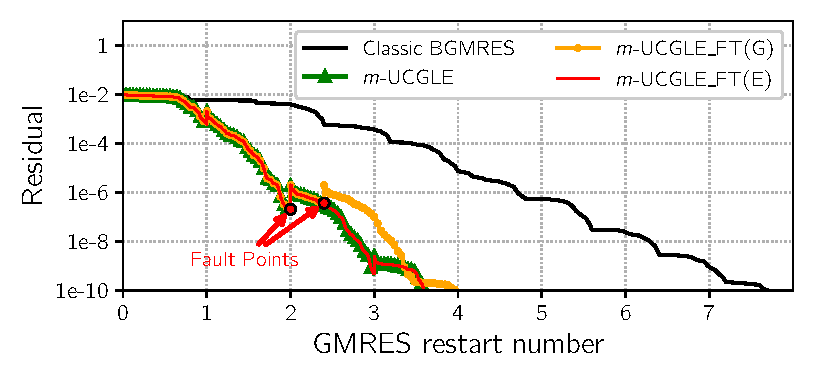
\includegraphics[width=.99\linewidth]{fig/convergence_ft.eps}
	\caption{Fault Tolerance Evaluation of $m$-UCGLE.}
	\label{fig:ft}
\end{figure}

The fault tolerance of $m$-UCGLE is studied by the simulation of the loss of either GMRES or $s$-KS Components. $m$-UCGLE\_FT(G) in Fig. \ref{fig:ft} represents the simulation of BGMRES in fault, and $m$-UCGLE\_FT(E) implies the fault simulation of $s$-KS. The curves of $m$-UCGLE and classic BGMRES represent the normal $m$-UCGLE and BGMRES without preconditioning respectively. 

The failure of $s$-KS Component is simulated by fixing the execution loop number of $s$-KS algorithm, it exits after a fixed number of iterations. We mark the $s$-KS fault point of tests in Fig. \ref{fig:ft}. The $m$-UCGLE\_FT(E) curves of the experimentations show that BGMRES Component will continue to solve the systems with LS preconditioning using the eigenvalues stored on the manager engine. There is not much difference between the curves of $m$-UCGLE\_FT(E) and $m$-UCGLE.

The failure of BGMRES Component (marked in Fig. \ref{fig:ft}) is simulated by fixing a small number of iterations before the achievement of convergence. We can find that after the fault of BGMRES Component, $s$-KS computing units will automatically take over the jobs of BGMRES component. This new BGMRES is recovered from the stat of the previous backup of the temporary solution $x_m$, and then continue to solve the linear systems with the checkpoint data.  Thus in the curve of UCGLE\_FT(G), the linear solver repeats a few steps of previous iterations from the fault point.


\section{Conclusions}

This chapter presents m-UCGLE, an extension of distributed and parallel method UCGLE to solve large-scale non-Hermitian sparse linear systems with multiple RHSs on modern supercomputers. $m$-UCGLE is implemented with three kinds of computational components which communicate by the asynchronous communication. A special engine is proposed to manger the communication and allocate multiple different components at the same time. $m$-UCGLE is able to accelerate the convergence, minimize the global communication, cover the synchronous points for solving linear systems with multiple RHSs on large-scale platforms. The experiments on supercomputers prove the good numerical and parallel performance of this method. $m$-UCGLE is implemented based on this novel paradigm on both homogeneous and heterogeneous clusters. This method is able to accelerate the convergence, minimize global communication, cover the synchronous points for solving linear systems with multiple RHSs on large-scale platforms. The experiments on supercomputers prove its good numerical and parallel performance. The fault tolerance and reusability of $m$-UCGLE is also proved by the simulation of failures of different components. Various parameters have impacts on the convergence. Thus, the auto-tuning scheme is required in the next step, where the systems can select the dimensions of Krylov subspace, the numbers of eigenvalues to be computed, the degrees of Least Squares polynomial according to different linear systems and cluster architectures. Different deflation and polynomial preconditioned iterative methods could be transformed according to this proposed paradigm, and further study should be done to compare them. A complete runtime for this paradigm should be developed to replace the prototype implementation of this chapter.

\clearemptydoublepage